\documentclass[twocolumn]{aastex63}

\usepackage{lipsum}

\let\tablenum\relax
\usepackage{siunitx}
\DeclareSIUnit\arcsec{as}
\DeclareSIUnit\solarmass{\ensuremath{M_\odot}}
\DeclareSIUnit\solarradius{\ensuremath{R_\odot}}
\DeclareSIUnit\solarlum{\ensuremath{L_\odot}}
\DeclareSIUnit\dex{dex}

\usepackage{graphicx}
% \graphicspath{{figures/}}
% \usepackage{amssymb}
% \usepackage{hyperref}

\newcommand{\numax}{\nu_\mathrm{max}}
\newcommand{\Dnu}{\Delta\nu}
\newcommand{\Yini}{Y_{\mathrm{ini}}}
\newcommand{\mlt}{\alpha_{\mathrm{MLT}}}
\newcommand{\metallicity}{[\mathrm{M} / \mathrm{H}]}
\newcommand{\Teff}{T_{\mathrm{eff}}}

\defcitealias{Serenelli.Johnson.ea2017}{S17}

% \received{June 1, 2019}
% \revised{January 10, 2019}
% \accepted{\today}

\begin{document}

\title{Modelling the first APOKASC sample of \textit{Kepler} dwarfs and subgiants using machine learning\\I. Project plan}
%\date{\today}
\author{Alex Lyttle}
\affiliation{University of Birmingham, Edgbaston, B15 2TT}

\begin{abstract}

Using grid based modelling to obtain fundamental stellar parameters is... However, such modelling methods suffer from systematic uncertainties... Interpolation can provide finer grid, but it brings about further systematics from the interpolation method. I present a project plan which aims to train an artificial neural network on at least one grid of stellar models. (neural networks trump interpolation because they learn the relationships between parameters by the adjusting of weights etc...) Coupled with a hierarchical Bayesian model, which allows for the sharing of parameters between stars, I will apply the method to the first APOKASC sample of Kepler dwarfs and subgiants.

\end{abstract}

\keywords{n/a}

\section{Introduction \& aims}


\begin{itemize}
    \item Problems with grid based modelling and interpolation
    \item What science does this limit? Ages, helium, mixing length
    \item Advantage of HBMs
    \item Advantage of neural networks and mention Guy's paper in prep?
    \item Refer to the Serenelli sample
    \item Goal of the project is to apply our method to a sample of asteroseismic dwarfs and maybe subgiants and compare results.
    \item Free up mixing length and helium abundance relation.
\end{itemize}

The scientific goals of this project are as follows:

\begin{itemize}
    \item Test the use of artificial neural networks to approximate the output of stellar models
    \item Determine stellar fundamentals for a sample of dwarfs and subgiants using a hierarchical Bayesian model which samples the trained neural network
    \item Probe the effects of freeing up parameters such as initial helium fraction and the mixing-length theory parameters on the stellar fundamentals and compare to \citetalias{Serenelli.Johnson.ea2017}
\end{itemize}

The main collaborators on this project are: Guy Davies (supervisor), Tanda Li (stellar models, MESA) and Lindsey Carboneau (neural networks). I also hope to seek help from other members of the group such as: Josefina Montalban (stellar models, \textit{Cley}) and Warrick Ball (details regarding \citetalias{Serenelli.Johnson.ea2017}). Some external collaborators who may be able to help include: Victor Silva Aguirre (comparisons with BASTA) and Jamie Tayar (gyrochronology considerations).

\section{Methods}

The methods for this project are split into three sections: data, grid and model. These

All code used in this project will be made publicly available upon submission. A private \textit{GitHub} repository has been made which will be made accessible to collaborators\footnote{\url{https://github.com/alexlyttle/kepler-dwarfs.git}}. 

\subsection{Data}\label{sec:data}

The objects being studied in this project are a subset of the first APOKASC catalog of \textit{Kepler} dwarfs and subgiant stars \citep[][hereafter \citetalias{Serenelli.Johnson.ea2017}]{Serenelli.Johnson.ea2017}. The full dataset comprises asteroseismology for 415 objects with respective fundamental parameters determined through grid based modelling (GBM) using two independent effective temperature scales: Sloan Digital Sky Survey (SDSS) \textit{griz} band photometric temperatures and APOGEE\footnote{Apache Point Observatory Galactic Evolution
Experiment} Stellar Parameters and Chemical Abundances Pipeline (ASPCAP) spectroscopic temperatures corresponding to Data Release 13 of SDSS.

I will not consider intermediate-mass stars (those with a convective core) and low-metallicity stars in this project. Therefore, I selected a subset of \citetalias{Serenelli.Johnson.ea2017} where stellar mass determined using each temperature scale lie in the range $0.85 < M/\si{\solarmass} < 1.15$ and metallicity from each scale is in the range $-0.3 < \metallicity < 0.3$. This subset contains 69 objects which are plot in Figure \ref{fig:subsample_hrd}. The values of surface gravity, $\log{g}$, and $\metallicity$ are determined for each temperature scale by \citetalias{Serenelli.Johnson.ea2017}. These plots show the subsample contains mostly main sequence stars and subgiants, with a few early red giant branch stars. Five 

\begin{deluxetable}{rrrrr}
\tablecaption{An extract from Table 3 of \citetalias{serenelliFirstAPOKASCCatalog-2017} comprising measurements of the global asteroseismic parameters from the Sydney pipeline \citep{huberAutomatedExtractionOscillation-2009} with uncertainties from the spread of results from several other pipelines.\label{tab:seismo}}
\tablehead{\colhead{\textit{Kepler} ID} & \colhead{$\nu_{\max}$} & \colhead{$\sigma_{\nu_{\max}}$} & \colhead{$\Delta\nu$} & \colhead{$\sigma_{\Delta\nu}$}}
\startdata
2450729 & 1053.105 & 114.904 & 61.910 & 2.539 \\
2991448 & 1111.248 & 18.148 & 61.732 & 0.899 \\
3223000 & 2573.222 & 563.234 & 110.919 & 1.662 \\
3241581 & 2807.592 & 395.565 & 123.412 & 2.821 \\
3427720 & 2726.381 & 56.767 & 120.045 & 0.120
\enddata
\end{deluxetable}


\begin{figure*}[htb!]
    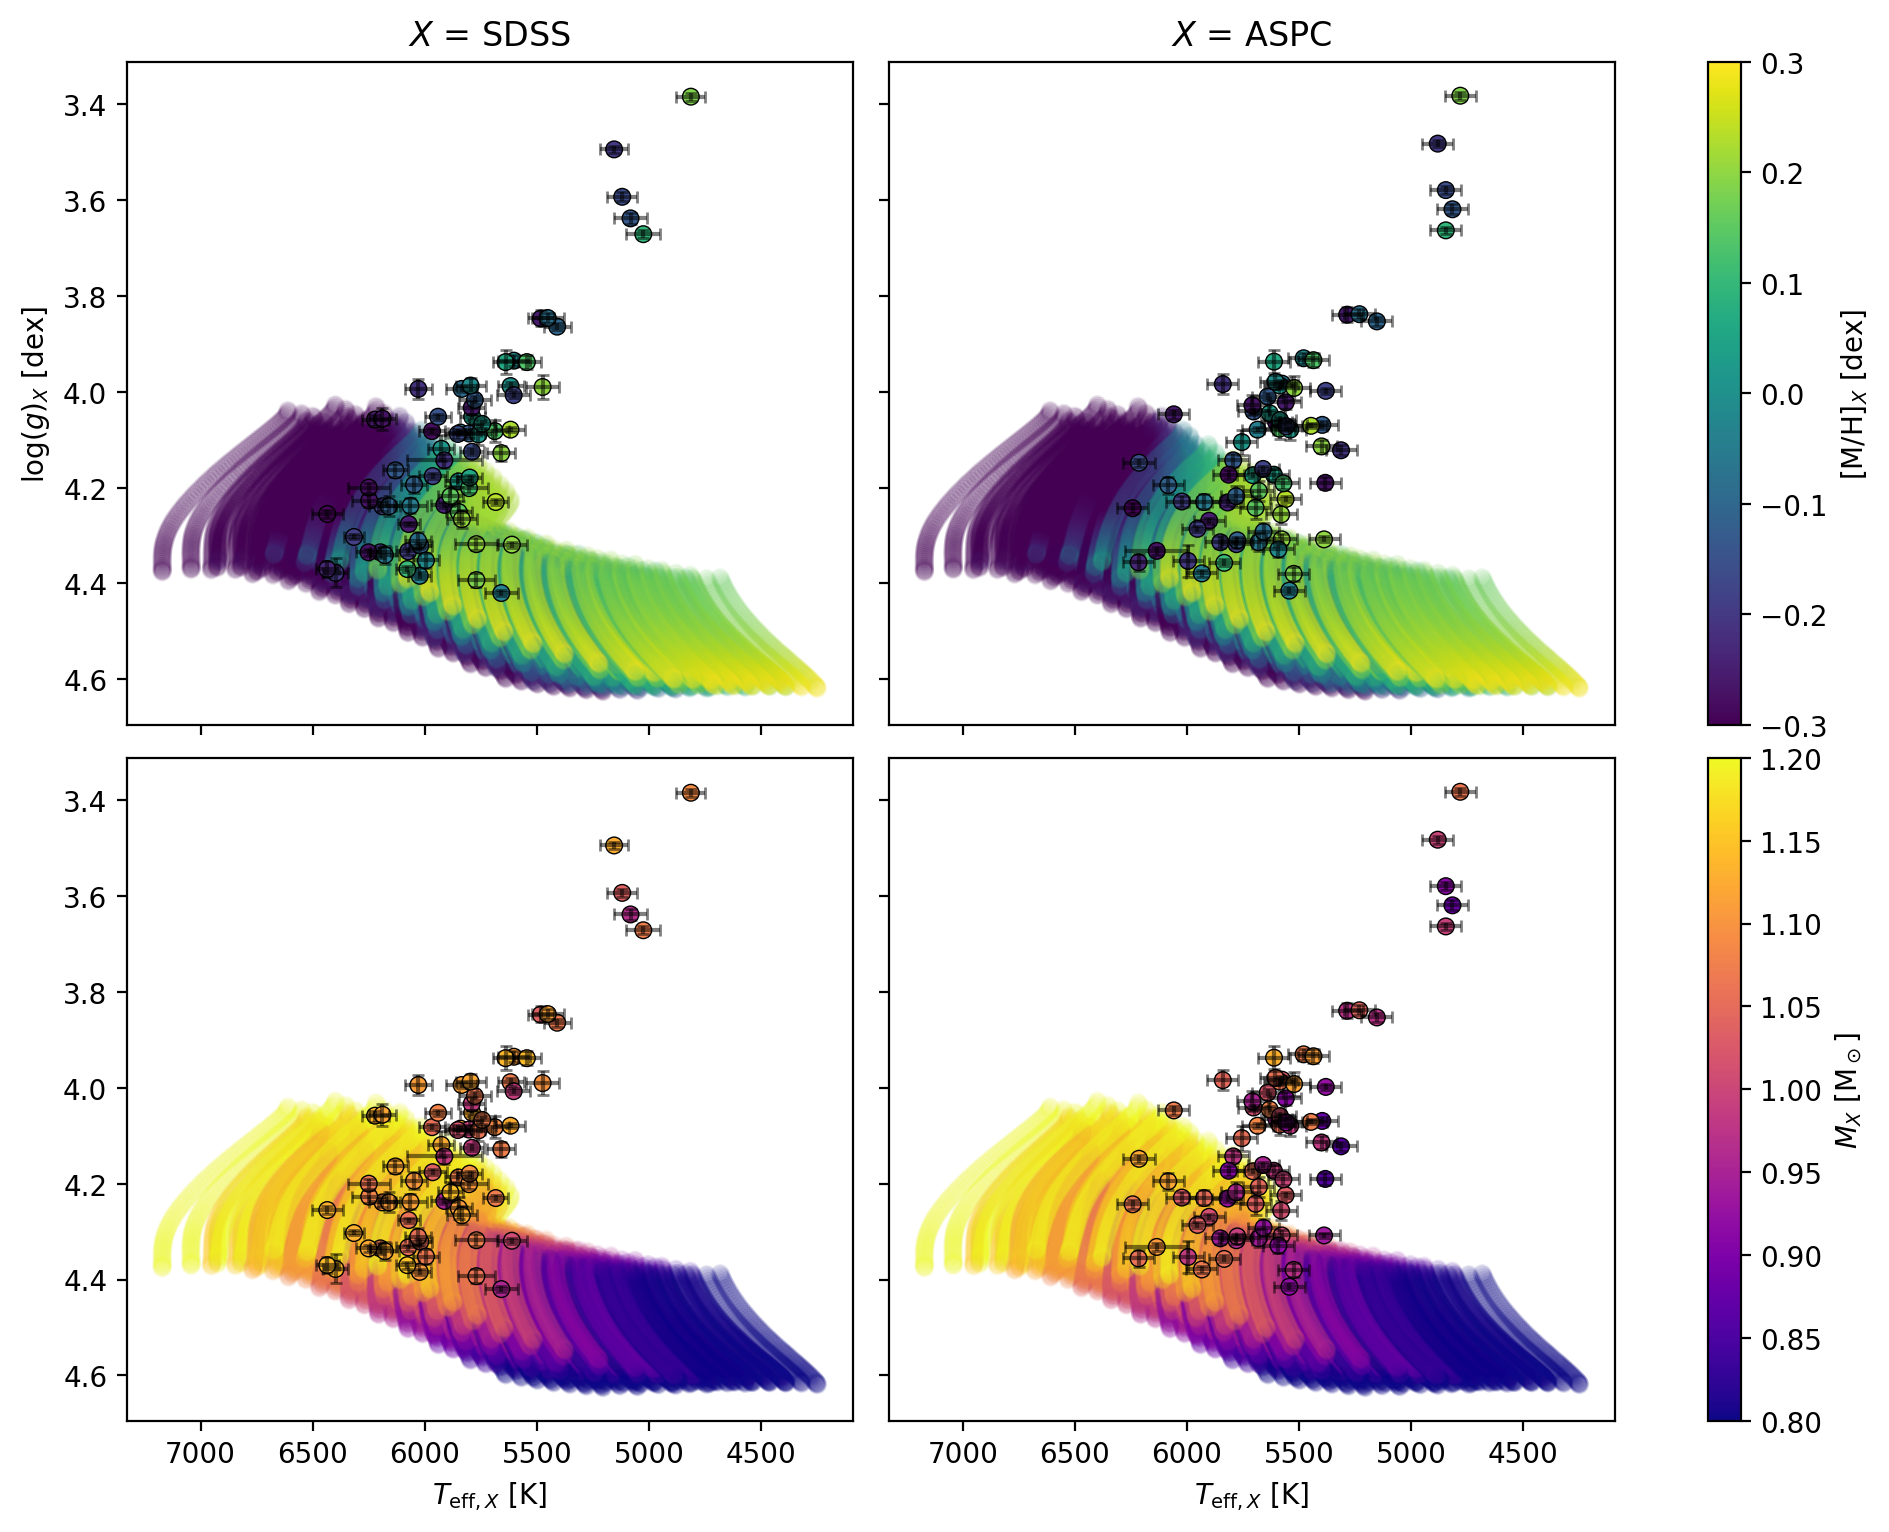
\includegraphics[width=1.0\textwidth]{figures/subsample_hrd.png}
    \caption{Results from a subsample of \citetalias{Serenelli.Johnson.ea2017} containing 69 low-mass objects. The plots comprise results which use SDSS \textit{griz} photometric temperatures (left) and ASPCAP spectroscopic temperatures from DR13 (right). The points in the background are from a grid of main sequence stellar models, \texttt{grid1\_sun}, described in Section \ref{sec:grid} with $\mlt = 1.9$ and $\Delta M = 0.04$. The data points are coloured by metallicity (top) and mass (bottom) corresponding to each temperature scale.}
    \label{fig:subsample_hrd}
\end{figure*}

\subsection{Grid}\label{sec:grid}

The span of the grid is chosen just outside the subset of \citetalias{Serenelli.Johnson.ea2017} chosen in \ref{sec:data}. The grid should be fine enough such that the neural network is able to learn the relationship between fundamentals and observables, but within a computational time of a few weeks. A grid (hereafter \texttt{grid1\_sun}) was computed by Tanda Li using MESA in late 2019. The models in \texttt{grid1\_sun}, which may be seen in \ref{fig:subsample_hrd}, were terminated at the main sequence turn-off. This figure shows that to include the more evolved stars, $\log(g) \lesssim 4.1$ the grid must be further evolved to at least the early red giant branch stage. I propose an extension to the initial conditions of \texttt{grid1\_sun} described below, with the bounds of \texttt{grid1\_sun} given in parentheses where appropriate,

\begin{eqnarray*}
    M / \si{\solarmass} \in [0.8, 1.2], &\quad& \Delta M = \SI{0.01}{\solarmass},\\
    \metallicity_{\mathrm{ini}} \in [-0.5\,(-0.3), 0.5\,(0.3)], &\quad& \Delta\metallicity_{\mathrm{ini}} = 0.1,\\
    \Yini \in [0.24, 0.32\,(0.3)], &\quad& \Delta\Yini = 0.01,\\
    \mlt \in [1.6\,(1.7), 2.3\,(2.0)], &\quad& \Delta\mlt = 0.1.
\end{eqnarray*}  

The bounds on mass are \SI{0.05}{\solarmass} outside of the range selected in the previous section. The upper bound is conveniently chosen as the point before which stars have a convective core, so there is no need to consider convective core overshooting. Median uncertainties on the masses determined by \citetalias{Serenelli.Johnson.ea2017} are $\sim \SI{6}{\percent}$, so a more conservative cut in mass of the dataset may be needed if we experience sampling issues due to being close to the edge of the grid. The bounds in initial metallicity are \SI{0.2}{\dex} outside of the dataset which comfortably covers the observed range by $\ga 3\sigma$. The grid will be computed with diffusion which affects the surface metallicity, reinforcing the need to extend $\metallicity_{\mathrm{ini}}$ beyond the data.

Since a primary focus of this project is to test the effects of freeing up $\mlt$ and $\Yini$, their bounds are chosen outside of the expected range of the dataset. For example, taking a helium enrichment ratio of $\Delta Y/ \Delta Z = 1.4$ \citep{brogaardAgeHeliumContent-2012} with upper and lower bounds from the literature of 1.0 and 1.8 respectively, gives approximate values of $\Yini$ between \num{0.25} and \num{0.31} for the initial metallicity bounds of the grid selected above. Therefore, the limits are chosen \num{0.01} outside this range. As for $\mlt$, I refer to hydrodynamical simulations \citep[e.g.][]{Trampedach.Stein.ea2014, Magic.Weiss.ea2015} to get a suitable range. For example, figure \ref{fig:mlt} suggests values between \num{1.7} and \num{2.2} to be a good choice of limits on $\mlt$. However, hydrodynamical simulations have been found to disagree with stellar codes using asteroseismic constraints \citep[e.g. see Fig. 9 of][]{SilvaAguirre.Lund.ea2017} so I have increased the limits by \num{0.1} above to account for these inconsistencies.

\begin{figure}[htb!]
    \centering
    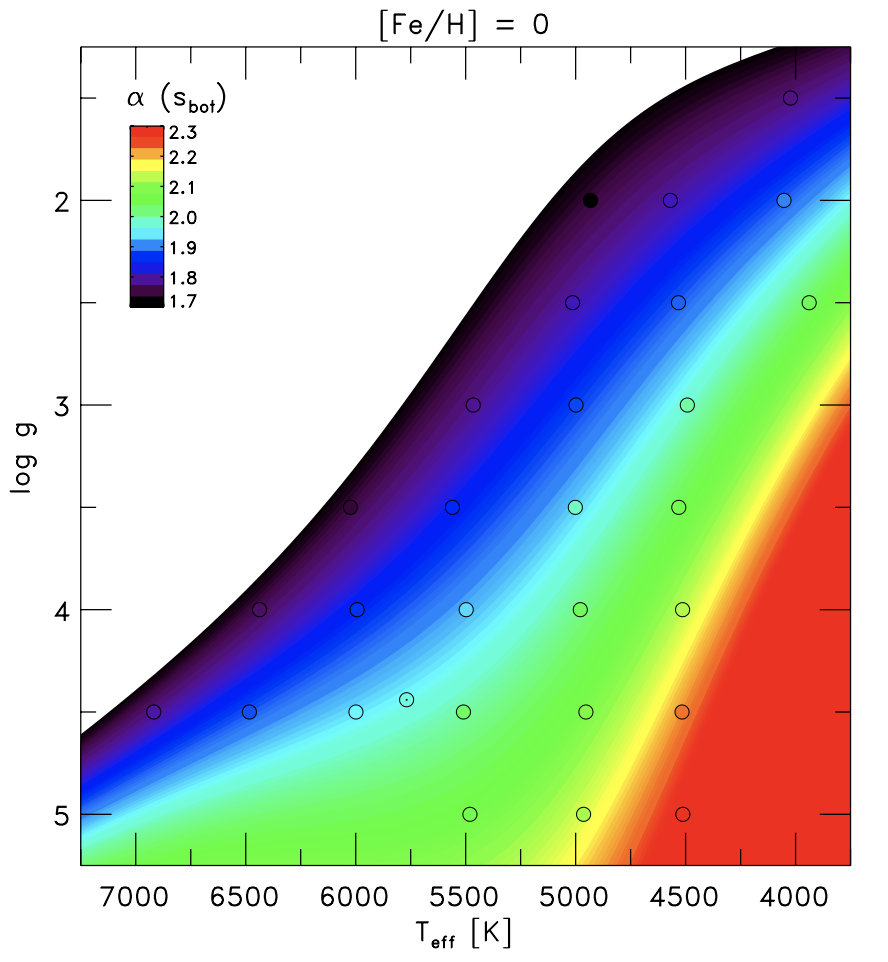
\includegraphics[width=0.4\textwidth]{figures/magic2015_mixing-length.png}
    \caption{Values of $\mlt$ from the hydrodynamical simulations of solar metallicity stars for position on the $\Teff - \log(g)$ plane. Source: Fig. 2 (\textit{left-panel}) of \citet{Magic.Weiss.ea2015}.}
    \label{fig:mlt}
\end{figure}

The purpose of the grid is to provide inputs and output to an artificial neural network (ANN) which will learn the relationship between the fundamental stellar input parameters (grid inputs) and the observables. These observables are some combination of the following: large frequency separation $\Dnu$, either from scaling relations or radial mode frequencies, effective temperature $\Teff$, surface metallicity $\metallicity$, radius $R/\si{\solarradius}$, and  luminosity $L/\si{\solarlum}$.

\subsection{Model}

The model will be split into two components: an ANN trained on the stellar grid, and a hierarchical Bayesian model (HBM) which shares hyper-parameters between stars in the subsample.

\subsubsection{Artificial neural network}

Output from each evolutionary track computed in Section \ref{sec:grid} will be combined into one master table. A random sample of \SI{20}{\percent} will be set aside for validation and the remaining \SI{80}{\percent} will be used for training the ANN. The training set will be resampled for mass steps of \SI{0.04}{\solarmass}, \SI{0.02}{\solarmass} and \SI{0.01}{\solarmass}. An ANN will be trained on all three datasets separately and evaluated to investigate the approximation ability with sparsity of the grid.

An off-grid validation dataset should also be computed, since the ANN inputs are discrete

The ANN will be a regression neural network with 5 to 10 fully-connected layers of $\sim 100$ neurons per layer. Finding the optimal network architecture will be achieved with a combination of a grid search and heuristic approach. A grid search will be used to find optimal start points for the learning rate, optimiser, activation function and regularisation. Once these are found, a trial and improvement method will be used to tune the best number of layers and neurons. To save time, tuning will be carried out on random subsamples of the data before being applied to the whole dataset.

Neural networks train better on inputs and outputs between -1 and 1. Positive ANN inputs and outputs may be log-normalised, either by taking the logarithm of the inputs and dividing by the median, or scaling by the log-mean and standard deviation. Similarly, some inputs may be normalised in linear space. To justify the normalisation method, histograms of input and output parameters should be plot. A selection of example ANN inputs and outputs from \texttt{grid1\_sun} are plot in Figure \ref{fig:hist}. For instance, these plots suggest parameters such as age and $\Dnu$ should be log-normalised whereas mass and metallicity may be scaled linearly.

\begin{figure*}[htb!]
    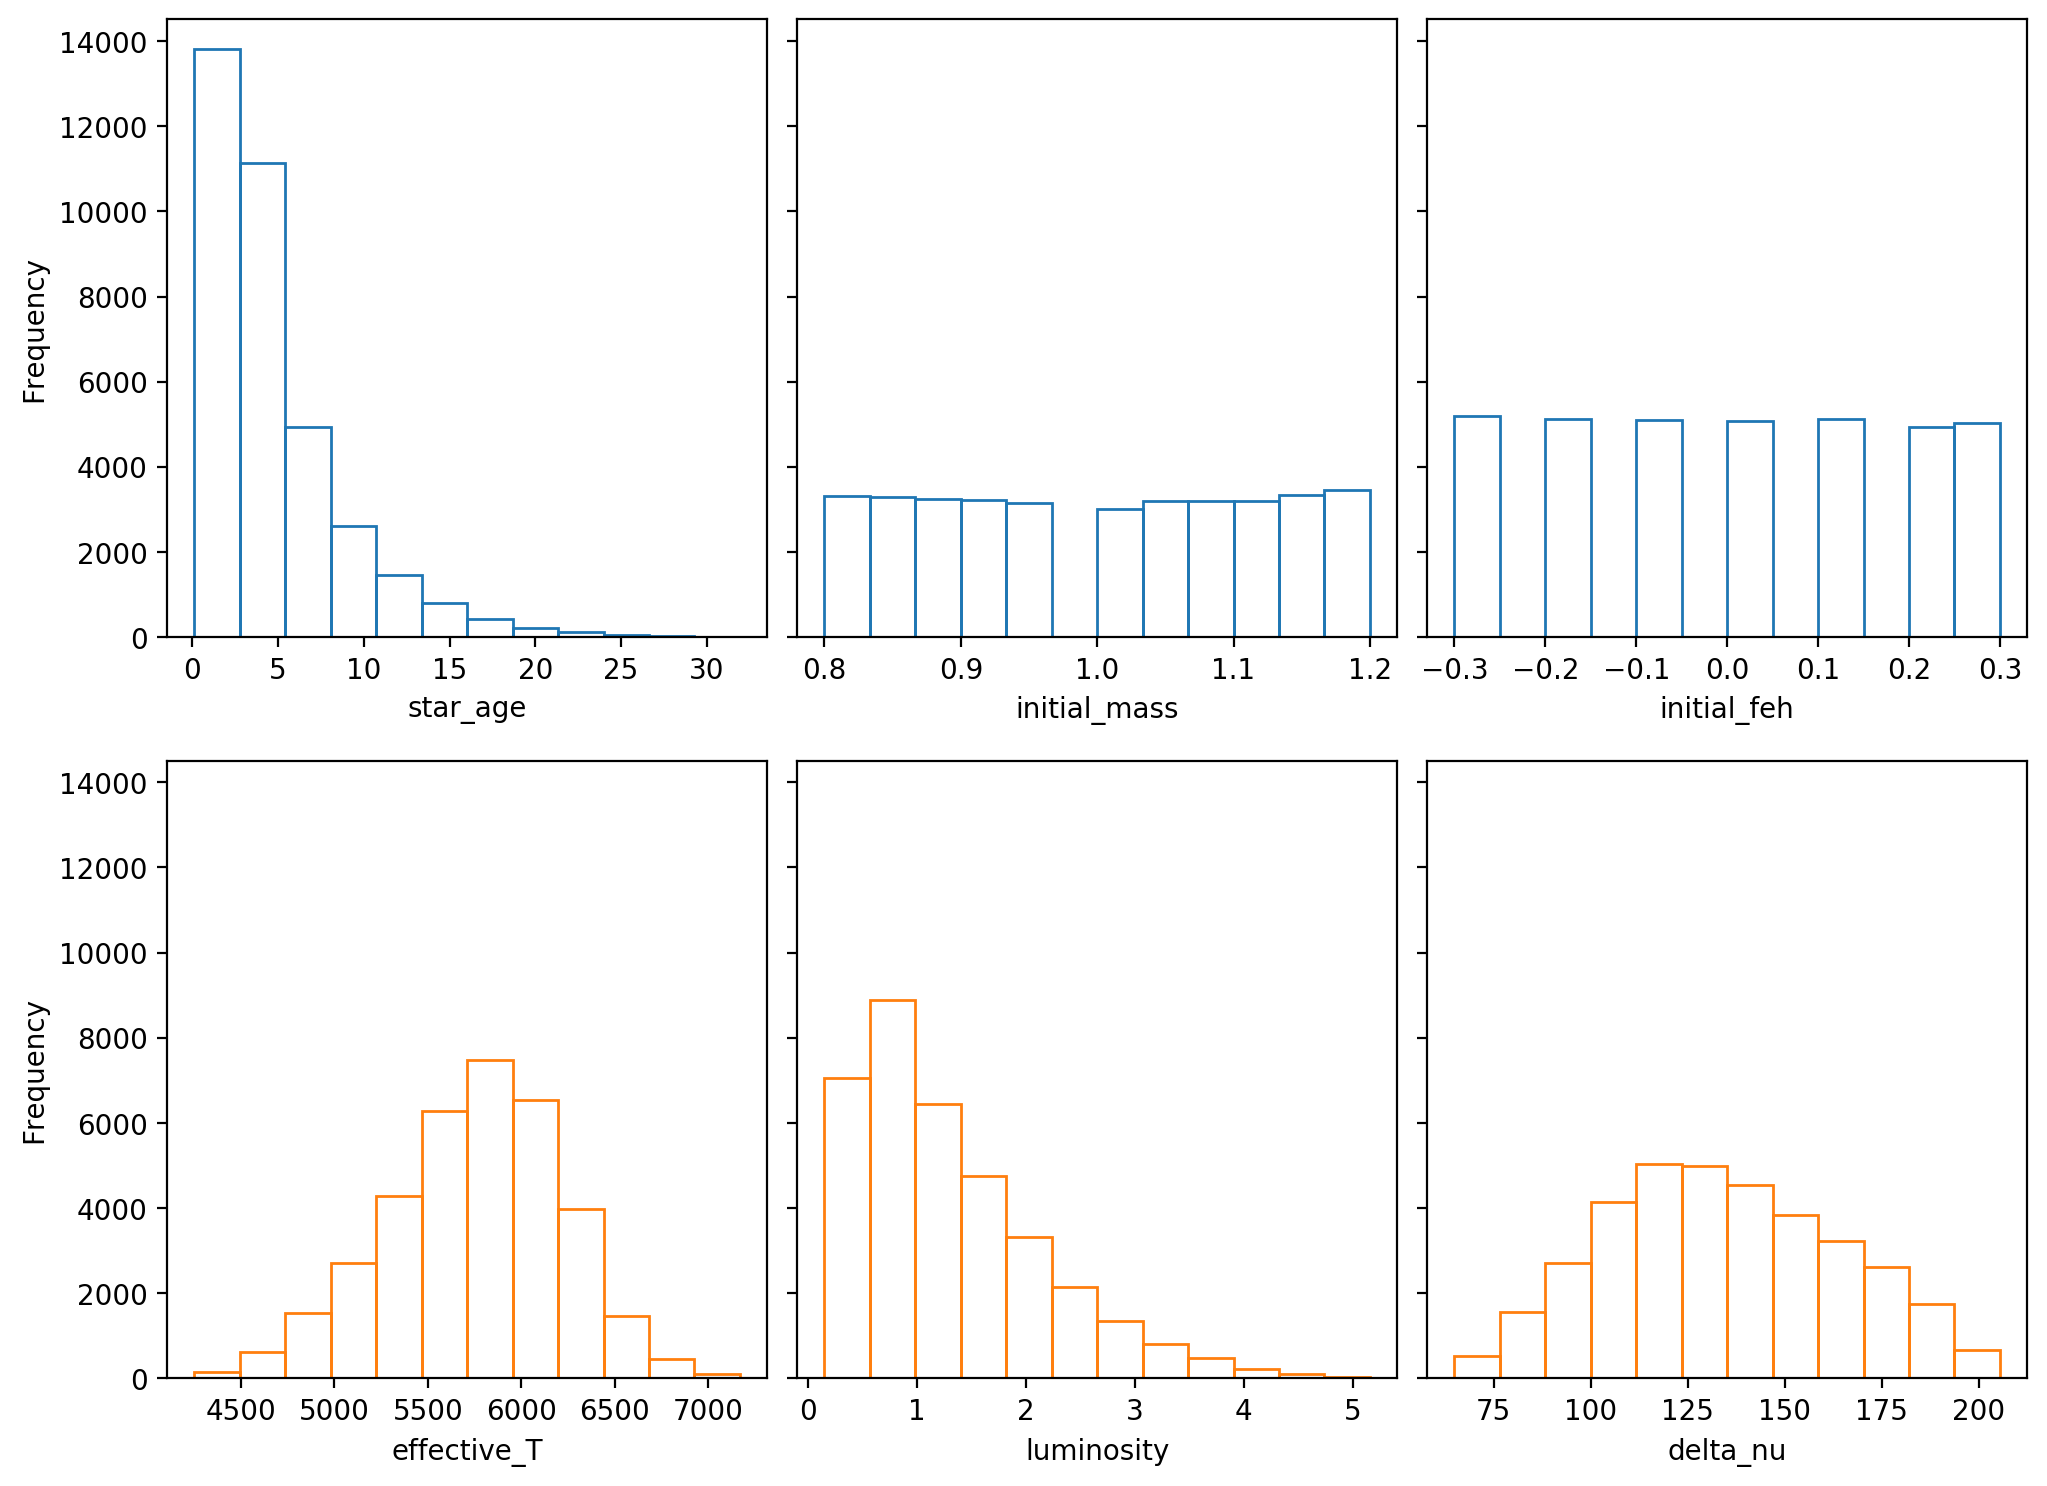
\includegraphics[width=1.0\textwidth]{figures/grid1_histogram.png}
    \caption{Histograms of selected columns in the output of \texttt{grid1\_sun} as examples of inputs (\textit{top}) and outputs (\textit{bottom}) to train the ANN.}
    \label{fig:hist}
\end{figure*}

\subsubsection{Hierarchical Bayesian model}

The HBM will be used to sample the function generated by the ANN given priors on the individual stellar fundamentals and hyperpriors on shared quantities which we expect to follow a particular distribution. For example, $\mlt$ could be allowed to vary between stars in one model and assume it follows a normal distribution across the sample in another. Additionally, $\Yini$ may be constrained to follow and enrichment law with $\Delta Y/\Delta Z$ as a hyperparameter, or left to vary freely.

\section{Plan}

The project plan is summarised in the following sections. I intend to make full use of \textit{GitHub} as a platform for organising this project. The milestones described in Section \ref{sec:comms} correspond to \textit{GitHub} milestones, which will be achieved via the completion of projects corresponding to those described in \ref{sec:timeline} each comprising one or more branches. 

\subsection{Timeline}\label{sec:timeline}

The plan is to complete the project by the end of June 2020. A gantt chart is presented in Figure \ref{fig:gantt} which breaks the project down into 9 sections and 5 milestones. The sections are as follows:

\begin{enumerate}
    \item Literature review -- I plan to read and understand \citetalias{Serenelli.Johnson.ea2017}, and compile and read papers which cover helium abundance and mixing-length theory, for example
    \item Compute grid of stellar models -- I will ask Tanda to compute a grid of stellar models as described in \ref{sec:grid}
    \item Cross-match dataset with \textit{Gaia} - I will cross-match the dataset with, for example \citet{Berger.Huber.ea2018} to get parallax-corrected distances for independent luminosities
    \item Preliminary method on MS stars -- I will apply the method to a small subset of the data which lie within \texttt{grid1\_sun}
    \item Train ANN on full grid -- I will work with Guy and Lindsey on training a neural network on the full grid
    \item Construct and run HBM -- working with Guy, I will construct and run an HBM using the trained ANN and observables
    \item Analyse results and uncertainties -- I will analyse the results and consider the effects of systematics (e.g. from the temperature scales)
    \item Review method and repeat -- I will present my results to colleagues and collaborators and revise the method if appropriate
    \item Write paper -- I will write a the paper and share with collaborators and co-authors when appropriate
\end{enumerate}

The milestones tie in with the communications strategy described in Section \ref{sec:comms}.

\begin{figure*}[htb!]
    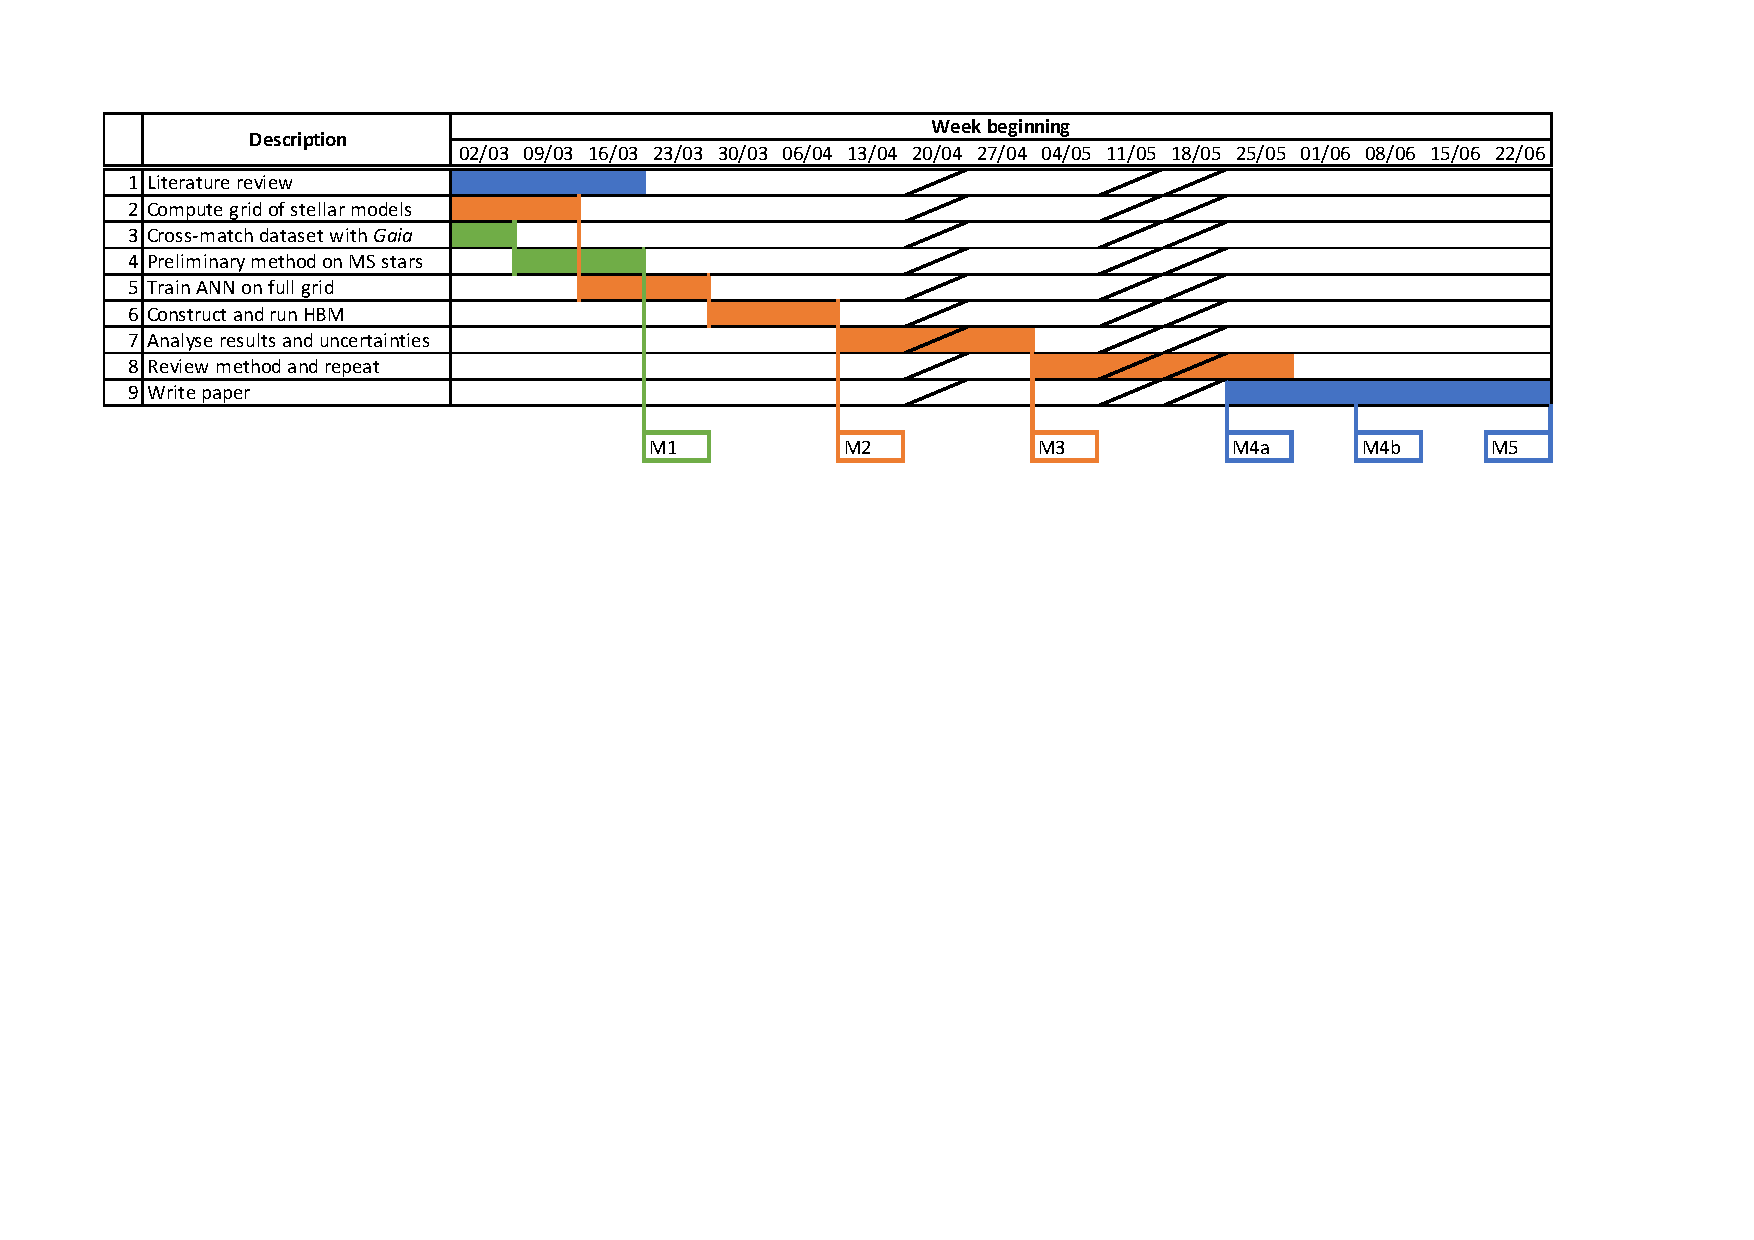
\includegraphics[width=1.0\textwidth,
    trim={1.5cm 13cm 3.1cm 0},clip]{figures/kepler-dwarfs_gantt.pdf}
    \caption{A gantt chart outlining 9 sections of the project and their dependencies. Each colour represents a dependency path through the project. Milestones are labelled by the letter M and described further in Section \ref{sec:timeline}. The shaded regions are weeks where I will be away from the University of Birmingham.}
    \label{fig:gantt}
\end{figure*}

\subsection{Communications strategy}\label{sec:comms}

Updates will be sent to project collaborators at each of the project milestones. The milestones are summarised as follows:

\renewcommand{\labelenumi}{M\arabic{enumi}.}
\begin{enumerate}
    \item 19th March 2020 -- Results from a test of the method will be sent to and discussed with collaborators. Feedback from here may be used to update the method
    \item 10th April 2020 -- Results from the HBM on the full dataset will be shared for discussion with collaborators
    \item 1st May 2020 -- A report or presentation summarising the results analysis should be made and given to collaborators.
    \item
    \begin{enumerate}
        \item 22nd May 2020 -- I will start writing the paper and share with other writers (e.g. Tanda for grid section)
        \item 5th June 2020 -- Send the paper to co-authors
    \end{enumerate}
    \item 27th June 2020 -- Submit the paper
\end{enumerate}
\renewcommand{\labelenumi}{\arabic{enumi}.}

These deadlines are marked in Figure \ref{fig:gantt} and represent key goals which need to be complete before moving forward.

\subsection{Risk and opportunity}

There are a number of risks and opportunities (abbreviated to opp.) associated with this project. For example,

\begin{itemize}
    \item[]
    \begin{itemize}
        \item[\textit{Risk:}] Grid does not fully cover the data (edge-effects in ANN and HBM)
        \item[\textit{Solution:}] Save MESA model files and extend grid further where necessary
    \end{itemize}
    \item[] 
    \begin{itemize}
        \item[\textit{Risk:}] Data loss
        \item[\textit{Solution:}] Make full use of version control and store grid output on the research data store (RDS)
    \end{itemize} 
\end{itemize}

\begin{itemize}
    \item[]
    \begin{itemize}
        \item[\textit{Opp.:}] Complete M2 ahead of schedule
        \item[\textit{Solution:}] Consider the effects of stellar model systematics by training on grids from different codes (e.g. \textit{Cley})
    \end{itemize}
    \item[]
    \begin{itemize}
        \item[\textit{Opp.:}]
        \item[\textit{Solution:}]
    \end{itemize}
\end{itemize}

\section{Summary}

\bibliography{references}{}
\bibliographystyle{aasjournal}

\end{document}
